% ============================================================
%  method.tex — TH-GNN paper, NeurIPS 2025
%  Source files consulted:
%    src/models/hgt.py, src/models/fusion.py
%    src/datasets/{base,movielens,amazon,yelp}.py
%    configs/paper_runs.yaml
% ============================================================

\section{Methodology}
\label{sec:method}

% ── Problem Formulation ───────────────────────────────────────────────────────
\subsection{Problem Formulation}
\label{sec:formulation}

Let $\mathcal{G}_t = (\mathcal{V}, \mathcal{E}_t)$ be a heterogeneous temporal
graph in which every node $v \in \mathcal{V}$ carries a type label
$\tau(v) \in \{\texttt{user}, \texttt{item}, \texttt{review}\}$ and every
directed edge $e = (s, d, t_e) \in \mathcal{E}_t$ carries a relation type
$\phi(e) \in \{\texttt{writes}, \texttt{about}, \texttt{rates}\}$ and a
Unix-second timestamp $t_e \in \mathbb{R}_{\geq 0}$.
We write $\mathcal{U}$, $\mathcal{I}$, $\mathcal{R}$ for the disjoint user,
item, and review node sets, so
$|\mathcal{V}| = |\mathcal{U}| + |\mathcal{I}| + |\mathcal{R}|$.
The three canonical relation types induce the edge partition
\begin{align}
  \mathcal{E}_{\texttt{writes}}
    &= \{(u, r,\, t_e) \mid u \in \mathcal{U},\; r \in \mathcal{R}\},
    \label{eq:ewrites} \\
  \mathcal{E}_{\texttt{about}}
    &= \{(r, i,\, t_e) \mid r \in \mathcal{R},\; i \in \mathcal{I}\},
    \label{eq:eabout} \\
  \mathcal{E}_{\texttt{rates}}
    &= \{(u, i,\, t_e) \mid u \in \mathcal{U},\; i \in \mathcal{I}\},
    \label{eq:erates}
\end{align}
with $\mathcal{E}_t =
  \mathcal{E}_{\texttt{writes}} \cup
  \mathcal{E}_{\texttt{about}}  \cup
  \mathcal{E}_{\texttt{rates}}$.
All three edge sets arising from a single review event share the same timestamp
$t_e$.

\textbf{Detection task.}
Each user carries a binary label $y_u \in \{0, 1\}$, where $y_u = 1$ denotes a
fake profile injected by a shilling attacker.
The objective is to learn a detector
\begin{align}
  f_\theta : \mathcal{G}_t \;\longrightarrow\; [0,1]^{|\mathcal{U}|}
  \label{eq:task}
\end{align}
producing per-user shilling scores $\hat{p}_u = f_\theta(u;\, \mathcal{G}_t)$,
with the binary prediction $\hat{y}_u = \mathbb{1}[\hat{p}_u > 0.5]$.

% ── Graph Construction ────────────────────────────────────────────────────────
\subsection{Heterogeneous Temporal Graph Construction}
\label{sec:graph_construction}

Each dataset is converted to $\mathcal{G}_t$ by a unified pipeline.
Raw interactions are filtered to the 5-core (users and items with at least five
interactions), sorted chronologically, and partitioned into train/val/test
windows by timestamp (70\,/\,10\,/\,20\,\%; shared across all detectors and
attacks).

\textbf{User node features.}
Each user $u$ is initialised with a structural feature vector
$\mathbf{x}_u \in \mathbb{R}^{D_u}$ whose first five components are computed
directly from the interaction log:
\[
  \mathbf{x}_u^{\text{base}} =
  \bigl[\deg(u),\; \bar{r}_u,\; \sigma_{r,u},\; \text{span}_u,\; \bar{\delta}_u\bigr],
\]
where $\deg(u)$ is the review count, $\bar{r}_u$ and $\sigma_{r,u}$ are the
mean and standard deviation of ratings, $\text{span}_u$ is the activity window
in days, and $\bar{\delta}_u$ is the mean inter-review gap in days.
Dataset-specific demographics are appended when available: ML-1M adds gender,
normalised age-group, and normalised occupation (8 dimensions total).

\textbf{Item node features.}
Items share the same five base statistics plus catalogue-level features:
ML-1M appends a normalised release year and an 18-dimensional genre multi-hot
(24 dimensions); Amazon datasets append $\log(1{+}\text{price})$, catalogue
average rating, and $\log(1{+}\text{review count})$ (8 dimensions); Yelp2018
appends business star rating, $\log(1{+}\text{review count})$, and an
is-open indicator (8 dimensions).

\textbf{Review node features.}
Each review node $r$ is assigned a scalar placeholder $x_r = 0$; its semantic
content is encoded separately by a frozen language model
(Section~\ref{sec:fusion}).

\textbf{Text embeddings.}
Review texts are encoded as frozen RoBERTa-base~\cite{liu2019roberta}
\texttt{[CLS]} vectors $\mathbf{e}_r \in \mathbb{R}^{768}$.
Item texts are constructed per dataset: ML-1M concatenates the movie title and
genre list; Amazon datasets concatenate the product title, up to five feature
bullets, and two description sentences; Yelp2018 concatenates the business name
and category string.
For ML-1M, which contains no review text, both the review and item CLS vectors
are set to $\mathbf{0}^{768}$, isolating the graph and temporal streams for
that dataset.
These node features are the input to the HGT encoder described next.

% ── HGT Encoder ──────────────────────────────────────────────────────────────
\subsection{HGT Encoder with Temporal Encoding}
\label{sec:hgt}

TH-GNN uses a two-layer Heterogeneous Graph Transformer
(HGT;~\cite{hu2020hgt}) as the structural backbone
(Figure~\ref{fig:architecture}).
Input features of each node type are first mapped to a shared hidden dimension
$D = 128$ by type-specific linear projections
$\mathbf{W}_{\mathrm{in}}^{\tau} \in \mathbb{R}^{D_\tau \times D}$.

\begin{figure*}[t]
  \centering
  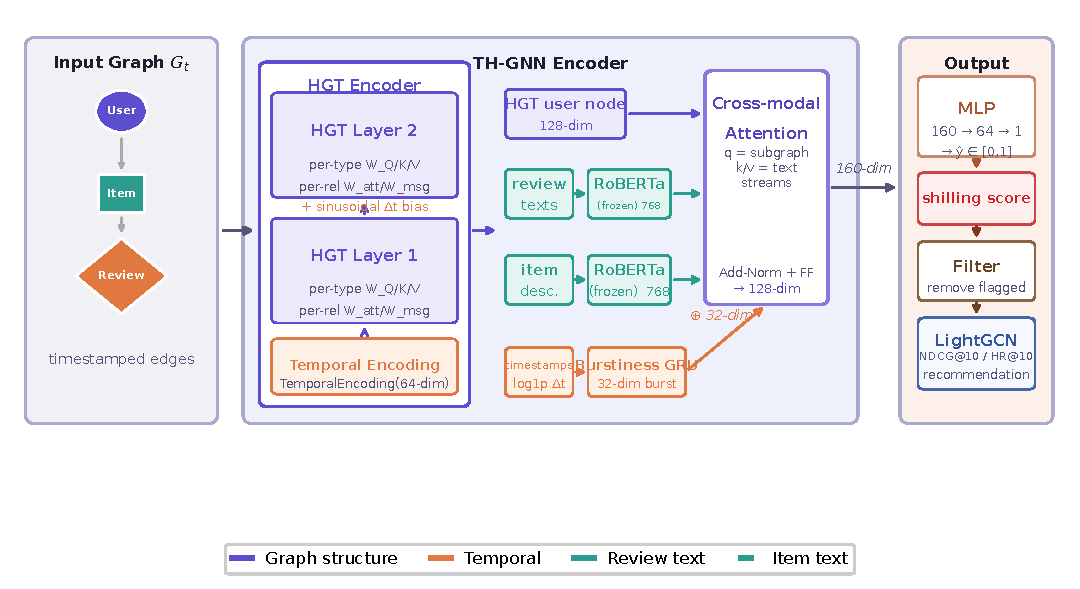
\includegraphics[width=\linewidth]{figures/architecture}
  \caption{TH-GNN architecture. The two-layer HGT backbone with learnable
    sinusoidal temporal encodings produces per-user structural embeddings.
    Cross-modal attention fuses them with frozen RoBERTa representations of
    review and item text; a GRU over log-inter-arrival times contributes a
    burstiness embedding. All streams are concatenated and passed to a
    two-layer MLP classifier.}
  \label{fig:architecture}
\end{figure*}

\textbf{Heterogeneous attention.}
At layer $l$, for each directed edge $e = (s, d)$ of relation type $\phi(e)$,
the per-head attention logit is
\begin{align}
  \mathrm{ATT}(s, e, d)
  &= \frac{1}{\sqrt{d_h}}
     \;\underbrace{
       \mathbf{q}(d)^{\!\top}
       \mathbf{W}_{\mathrm{att}}^{\phi(e)}
       \mathbf{k}(s)
     }_{\text{relation-specific bilinear}}
     \;+\; \varphi(\Delta t_{sd}),
  \label{eq:att}
\end{align}
where $d_h = D / H = 32$ is the per-head dimension ($H = 4$ heads) and the
query, key, and value projections are type-specific:
\begin{align}
  \mathbf{q}(d) &= \mathbf{W}_Q^{\tau(d)} \mathbf{h}_d^{(l)}, &
  \mathbf{k}(s) &= \mathbf{W}_K^{\tau(s)} \mathbf{h}_s^{(l)}, &
  \mathbf{v}(s) &= \mathbf{W}_V^{\tau(s)} \mathbf{h}_s^{(l)}.
  \label{eq:qkv}
\end{align}
The per-relation weight $\mathbf{W}_{\mathrm{att}}^{\phi(e)} \in
\mathbb{R}^{H \times d_h \times d_h}$ learns a distinct interaction pattern
for each of the three edge types.
Softmax is computed jointly over \emph{all} incoming edges of node $d$,
irrespective of edge type, before weighting the relation-specific messages
$\mathrm{MSG}(s, e, d) = \mathbf{W}_{\mathrm{msg}}^{\phi(e)} \mathbf{v}(s)$.
The output is formed by aggregation, output projection, and residual layer
normalisation:
\begin{align}
  \mathrm{Agg}(d)
  &= \sum_{(s,e) \in \mathcal{N}(d)}
     \mathrm{softmax}\!\bigl[\mathrm{ATT}(s, e, d)\bigr]
     \cdot \mathrm{MSG}(s, e, d),
  \label{eq:agg} \\
  \mathbf{h}_d^{(l+1)}
  &= \mathrm{LayerNorm}\!\left(
       \mathbf{W}_{\mathrm{out}}^{\tau(d)}\,
       \mathrm{GELU}\!\left(\mathrm{Agg}(d)\right)
       + \mathbf{W}_{\mathrm{res}}^{\tau(d)}\,
       \mathbf{h}_d^{(l)}
     \right).
  \label{eq:update}
\end{align}

\textbf{Relative temporal encoding.}
The scalar bias $\varphi(\Delta t_{sd})$ in Equation~\eqref{eq:att} injects the
elapsed time between interacting events directly into the attention logit,
without altering node feature dimensions.
Let $\Delta t_{sd} = |t_s - t_d|$ (seconds).
The encoding uses learnable sinusoidal frequencies:
\begin{align}
  \varphi(\Delta t)
  = \mathbf{w}_p^{\!\top}
    \begin{bmatrix}
      \sin\!\left(\boldsymbol{\omega} \cdot \tfrac{\Delta t}{86400}
                  + \boldsymbol{\psi}\right) \\[2pt]
      \cos\!\left(\boldsymbol{\omega} \cdot \tfrac{\Delta t}{86400}
                  + \boldsymbol{\psi}\right)
    \end{bmatrix},
  \label{eq:temporal}
\end{align}
where $\boldsymbol{\omega}, \boldsymbol{\psi} \in \mathbb{R}^{d_T/2}$ are
learnable frequencies and phases ($d_T = 64$) and $\mathbf{w}_p \in
\mathbb{R}^{d_T}$ is a learned projection vector.
Time deltas are normalised to days to keep initial frequency values near zero
meaningful; $\mathbf{w}_p$ and its bias are zero-initialised so the temporal
term starts at zero and grows only as the loss demands.

% ── Multimodal Fusion ─────────────────────────────────────────────────────────
\subsection{Multimodal Fusion}
\label{sec:fusion}

After $L = 2$ HGT layers, each user $u$ has a structural embedding
$\mathbf{h}_u^{(L)} \in \mathbb{R}^D$.
TH-GNN combines this with two text streams and a burstiness stream before
the classification head (Figure~\ref{fig:architecture}).

\textbf{Three input streams.}
\begin{enumerate}[leftmargin=1.8em,itemsep=1pt]
  \item \emph{Graph stream.}
        The HGT user node output
        $\mathbf{h}_u^{(L)} \in \mathbb{R}^{128}$.
  \item \emph{Review text stream.}
        Mean-pooled RoBERTa \texttt{[CLS]} vectors over the user's reviews:
        $\mathbf{r}_u
          = \tfrac{1}{|\mathcal{R}_u|}
            \sum_{r \in \mathcal{R}_u} \mathbf{e}_r
          \in \mathbb{R}^{768}$.
  \item \emph{Item text stream.}
        Mean-pooled RoBERTa \texttt{[CLS]} vectors of items reviewed by $u$:
        $\mathbf{z}_u
          = \tfrac{1}{|\mathcal{R}_u|}
            \sum_{r \in \mathcal{R}_u} \mathbf{e}_{i(r)}
          \in \mathbb{R}^{768}$,
        where $i(r)$ is the item covered by review $r$.
\end{enumerate}
All three streams are projected to a shared dimension $d_p = 128$ via
type-specific linear maps $\mathbf{W}_{\mathrm{sub}}$, $\mathbf{W}_{\mathrm{rev}}$,
$\mathbf{W}_{\mathrm{item}}$:
\[
  \tilde{\mathbf{h}}_u = \mathbf{W}_{\mathrm{sub}}\mathbf{h}_u^{(L)}, \quad
  \tilde{\mathbf{r}}_u = \mathbf{W}_{\mathrm{rev}}\mathbf{r}_u, \quad
  \tilde{\mathbf{z}}_u = \mathbf{W}_{\mathrm{item}}\mathbf{z}_u.
\]

\textbf{Cross-modal attention.}
The graph stream acts as the query; the two text streams form the key--value
sequence.
The fused representation is produced by a transformer block with a single query
token:
\begin{align}
  \tilde{\mathbf{f}}_u,\; \boldsymbol{\alpha}_u^{\mathrm{txt}}
  &= \mathrm{MHA}\!\left(
       \tilde{\mathbf{h}}_u,\;\;
       \bigl[\tilde{\mathbf{r}}_u;\; \tilde{\mathbf{z}}_u\bigr],\;\;
       \bigl[\tilde{\mathbf{r}}_u;\; \tilde{\mathbf{z}}_u\bigr]
     \right), \label{eq:crossattn} \\[3pt]
  \mathbf{q}_u'
  &= \mathrm{LN}\!\left(\tilde{\mathbf{h}}_u + \tilde{\mathbf{f}}_u\right), \label{eq:addnorm1} \\
  \mathbf{f}_u
  &= \mathrm{LN}\!\left(\mathbf{q}_u' + \mathrm{FF}(\mathbf{q}_u')\right)
    \in \mathbb{R}^{d_p}, \label{eq:fusionout}
\end{align}
where $\mathrm{MHA}$ uses $H = 4$ heads, $\boldsymbol{\alpha}_u^{\mathrm{txt}}
\in \mathbb{R}^2$ is the learned attention distribution over the review and item
streams, and $\mathrm{FF}$ is a two-layer position-wise feed-forward network
(hidden size $4 d_p$, GELU activation).

\textbf{Temporal burstiness GRU.}
Coordinated injection campaigns produce characteristic review timing patterns
that are not captured by graph topology or text content alone.
For user $u$ with reviews at sorted timestamps $t_1 < t_2 < \cdots < t_{L_u}$,
we compute the log-inter-arrival sequence
\begin{align}
  \mathbf{b}_u^{\mathrm{in}}
  = \bigl[
      \log(1 + t_2 - t_1),\;
      \log(1 + t_3 - t_2),\;
      \ldots,\;
      \log(1 + t_{L_u} - t_{L_u - 1})
    \bigr]
  \label{eq:iat}
\end{align}
and encode it with a single-layer GRU (hidden size 32):
$\mathbf{b}_u = \mathrm{GRU}(\mathbf{b}_u^{\mathrm{in}}) \in \mathbb{R}^{32}$.
Users with fewer than two reviews receive $\mathbf{b}_u = \mathbf{0}^{32}$.

\textbf{Classification head.}
The fused representation and the burstiness vector are concatenated and passed
through a two-layer MLP with a LayerNorm input gate:
\begin{align}
  \mathbf{c}_u   &= [\mathbf{f}_u;\; \mathbf{b}_u] \in \mathbb{R}^{160},
  \label{eq:concat} \\
  \hat{p}_u      &= \sigma\!\left(
                      \mathbf{W}_2\;
                      \mathrm{GELU}\!\left(
                        \mathbf{W}_1\, \mathrm{LN}(\mathbf{c}_u)
                      \right)
                    \right),
  \label{eq:mlp}
\end{align}
where $\mathbf{W}_1 \in \mathbb{R}^{64 \times 160}$,
$\mathbf{W}_2 \in \mathbb{R}^{1 \times 64}$, and $\sigma$ is the sigmoid.
We train the full model end-to-end using the focal loss objective described next.

% ── Training Objective ────────────────────────────────────────────────────────
\subsection{Training Objective}
\label{sec:objective}

\textbf{Class imbalance.}
Shilling attacks are sparse by design.
At our lowest injection rate (0.5\,\%), the genuine-to-fake user ratio reaches
$200\!:\!1$ on ML-1M (${\approx}30$ injected profiles among 6\,040 users).
Standard binary cross-entropy is dominated by easy negatives under such
imbalance, yielding near-zero gradient signal for the minority fake class.

\textbf{Focal loss.}
We replace cross-entropy with the binary focal
loss~\cite{lin2017focal}, which down-weights well-classified negatives via a
modulating factor $(1 - p_t)^\gamma$:
\begin{align}
  \mathcal{L}_{\mathrm{FL}}
  = -\frac{1}{|\mathcal{B}|}
    \sum_{u \in \mathcal{B}}
    \alpha_t \left(1 - p_t\right)^{\!\gamma} \log p_t,
  \label{eq:focal}
\end{align}
where $\mathcal{B}$ is the training mini-batch and
\begin{align}
  p_t
  = \begin{cases}
      \hat{p}_u      & \text{if } y_u = 1, \\
      1 - \hat{p}_u  & \text{if } y_u = 0,
    \end{cases}
  \qquad
  \alpha_t
  = \begin{cases}
      \alpha      & \text{if } y_u = 1, \\
      1 - \alpha  & \text{if } y_u = 0.
    \end{cases}
  \label{eq:pt_at}
\end{align}
We set $\gamma = 2.0$ and $\alpha = 0.25$.
At a moderately confident prediction of $p_t = 0.5$, the factor
$(1 - p_t)^2 = 0.25$ reduces the contribution of easy negatives by $4\times$
relative to cross-entropy, concentrating gradient mass on rare fake profiles
and on ambiguous boundary cases.
At $p_t = 0.9$ (a confidently correct genuine-user prediction), the factor
falls to $0.01$, contributing negligibly to the loss.

\textbf{Optimisation.}
The model is trained end-to-end with Adam
($\text{lr} = 10^{-3}$, weight decay $10^{-4}$, batch size 512) for up to
100 epochs; training terminates early when validation
F\textsubscript{1} does not improve for 10 consecutive epochs.
RoBERTa weights are frozen throughout.
